\documentclass[10pt]{beamer}
\usepackage{anyfontsize}
\usepackage{minted}
\usepackage[T1]{fontenc}

\usepackage[style=british]{csquotes}

\def\signed #1{{\leavevmode\unskip\nobreak\hfil\penalty50\hskip1em
  \hbox{}\nobreak\hfill #1%
  \parfillskip=0pt \finalhyphendemerits=0 \endgraf}}

\newsavebox\mybox
\newenvironment{aquote}[1]
  {\savebox\mybox{#1}\begin{quote}\openautoquote\hspace*{-.7ex}}
  {\unskip\closeautoquote\vspace*{1mm}\signed{\usebox\mybox}\end{quote}}

\title[G-NODE FOSDEM]{G-Node Goes to FOSDEM}
\author{Achilleas Koutsou \& Michael Sonntag}
\date{March 05, 2018}

\graphicspath{{./figures/}{./photos/}}

\begin{document}

\maketitle

\begin{frame}{FOSDEM}
    \begin{center}
        \textbf{F}ree and \textbf{O}pen \textbf{S}ource Software \textbf{D}evelopers' \textbf{E}uropean \textbf{M}eeting
    \begin{figure}
        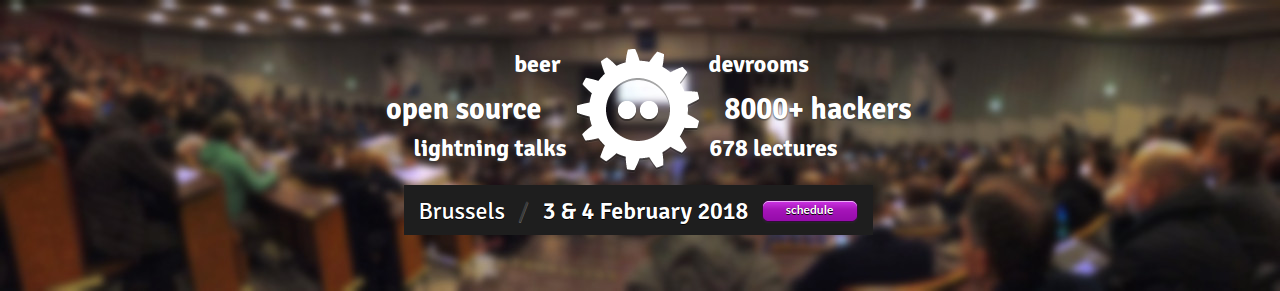
\includegraphics[width=\textwidth]{FOSDEM-banner.png}
    \end{figure}
    \end{center}

\end{frame}

\begin{frame}{FOSDEM}{About}
    Since 2001
    \begin{aquote}{FOSDEM about page}
        [\ldots] a two-day event organised by volunteers to promote the widespread use of free and open source software.
    \end{aquote}

    \begin{itemize}
        \item When: First weekend of February (every year)
        \item Where: ULB Campus du Solbosch Av. F. D. Roosevelt 50 1050 Bruxelles Belgium (every year)
        \item Registration: Free, no registration necessary (every year)
        \item Size: 8000+ estimated attendees (and growing (every year)), 678 lectures in 2 days
    \end{itemize}
\end{frame}

\begin{frame}{Motivation and rationale}{Brussels}
    \begin{enumerate}
        \item \href{./photos/beer.jpg}{Beer $\bullet$}
        \item \href{./photos/chocoballs.jpg}{Chocolate $\bullet$}
        \item Meeting FOSS developers
        \item Attending talks on FOSS
    \end{enumerate}
    For updates and inspiration for our own projects.
\end{frame}

\begin{frame}{Motivation and rationale}{Conference}
    The serious reasons
    \begin{itemize}
        \item Learn about advances in programming languages and technologies
        \item Devrooms (tracks) dedicated to languages and technologies we use:
            \begin{itemize}
                \item Go devroom: \href{./photos/go-devroom-queue.jpg}{Perhaps the most popular room this year $\bullet$}
                \item \href{./photos/python-talk.jpg}{Python main track $\bullet$}
            \end{itemize}
        \item General interest devrooms:
            \begin{itemize}
                \item Community devroom: Engaging with project communities to build better software
                \item Hardware Enablement devroom: Improving Linux hardware support (\href{./photos/kellner-talk.jpg}{with a \emph{fascinating} talk by the infamous \emph{Christian Kellner} $\bullet$})
            \end{itemize}
        \item Meeting people:
            \begin{itemize}
                \item Collaborators
                \item \href{./photos/collab.jpg}{Developers and maintainers of projects we use and find interesting $\bullet$}
            \end{itemize}
    \end{itemize}
\end{frame}

\begin{frame}{FOSDEM overview}{General Highlights and Topics}
    \begin{figure}
        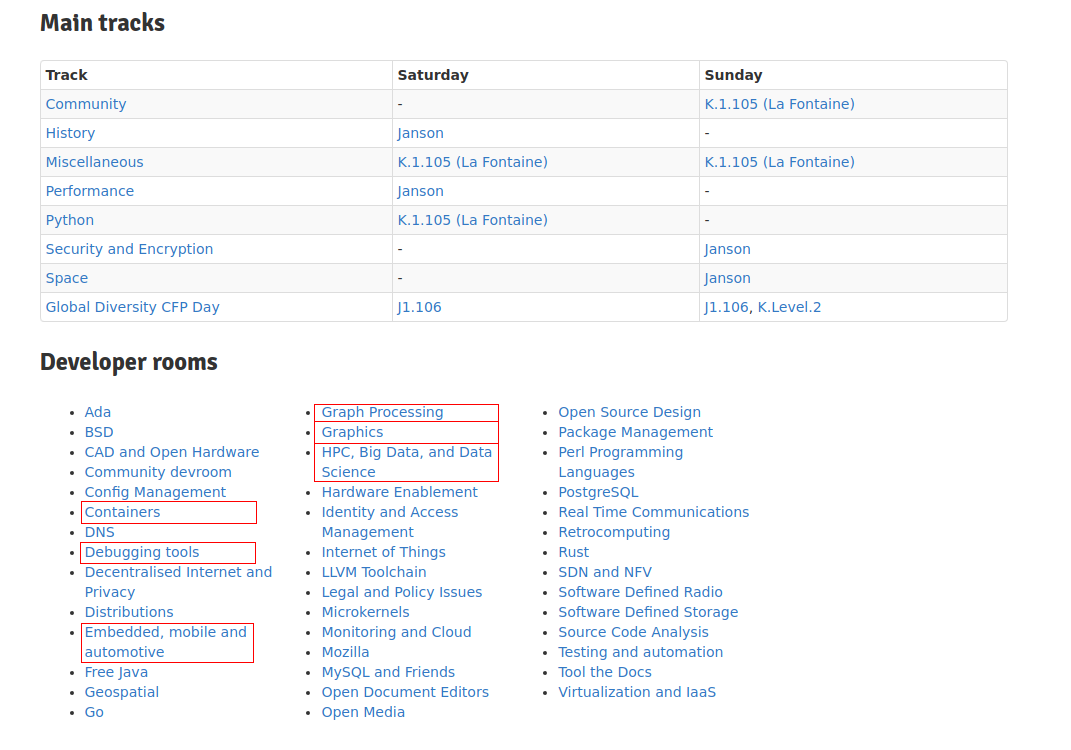
\includegraphics[width=\textwidth]{tracks-devrooms.png}
    \end{figure}

    FOSDEM tracks: \url{https://fosdem.org/2018/schedule/tracks}
\end{frame}

\begin{frame}{FOSDEM overview}{Other events}
    \begin{itemize}
        \item Linux and FOSS Certification exams
        \item Fringe events: Independently organised peripheral events
            \begin{itemize}
                \item Great for in-depth conversations about specific projects or topics
            \end{itemize}
        \item Lightning talks: Mostly scheduled but often allow last-minute additions about various topics
        \item Booths and exhibitions
        \begin{itemize}
            \item \href{./photos/stickers.jpg}{Popular open source projects and distributions $\bullet$}
            \item \href{./photos/booths.jpg}{Community booths $\bullet$}
            \item \href{./photos/merch.jpg}{Merch \& Swag $\bullet$}
        \end{itemize}
    \end{itemize}
\end{frame}

\begin{frame}{Go there}{Here's why}
    \begin{itemize}
        \item Talks that might be interesting for your work
        \item Meet developers of projects you are using (or plan to use)
        \item Expand your horizons: Discover new projects and tools that could be useful for you
        \item Show off your own (hardware) projects: Get developers interested and turn them into contributors
        \item Host your own devroom (e.g., FOSS research tools and methodologies)
        \item \href{./photos/github-coffee.jpg}{Free coffee, from GitHub with love $\bullet$}
        \item SUPPORT FREE OPEN SOURCE SOFTWARE (because it supports you)
    \end{itemize}
\end{frame}

\begin{frame}{FOSDEM Survival Guide}{Tips \& Tricks}
    \begin{itemize}
        \item Plan ahead: True for any conference, but FOSDEM tends to be \href{./photos/room-full.jpg}{slightly busier $\bullet$}
        \item On the other hand, all talks are streamed live and archived [\url{https://fosdem.org/2018/schedule/events/}]
            \begin{itemize}
                \item Archived talks are available from previous years
                \item Yes, you \emph{can} stream talks from home, but you can't ask questions or discuss issues with the speakers/community
            \end{itemize}
        \item Several companion apps available for iOS \& Android: Support scheduling, bookmarking, map, and room availability
        \item Stay in one room if interested in a future talk; you might not be able to get in if you leave (varies by topic)
        \item Make sure your EDUROAM account is working! The conference provides free WiFi, but the university's Eduroam network is much more reliable
        \item Enjoy and have fun
    \end{itemize}
\end{frame}

\begin{frame}{FOSDEM}{2019}
    \begin{center}
        THANK YOU FOR YOUR ATTENTION

        SEE YOU IN BRUSSELS NEXT YEAR
    \end{center}
\end{frame}

\begin{frame}{FOSDEM}{Resources}
    Resources

    \begin{itemize}
        \item FOSDEM 2018: \url{https://fosdem.org/2018}
    \end{itemize}
\end{frame}

\end{document}
